\documentclass{standalone}

\usepackage{tikz}
\usetikzlibrary{positioning, fit,  shapes.geometric}
\usepackage{ifthen}
\usepackage{etoolbox}

\tikzset{
	backgroundcolor/.style ={fill=white},
	every node/.append style={
		minimum height=7mm,
	},
	labe/.append style={
		%Blue,
		align = center,
		backgroundcolor,
		fill opacity=0.6,
		text opacity=1,
		font={\footnotesize\itshape}	
	},
	layer/.append style={
		draw,
		align = center,
		minimum height=7mm,
	},
	tight/.append style={
		inner sep=0.2mm,
	},
	lookupbox/.append style={
		draw=none,
		append after command={
		       	[shorten <= -0.5\pgflinewidth]
		       	([shift={(-1.5\pgflinewidth,-0.5\pgflinewidth)}]\tikzlastnode.north east)
		       	edge([shift={( 0.5\pgflinewidth,-0.5\pgflinewidth)}]\tikzlastnode.north west) 
		       	([shift={( 0.5\pgflinewidth,-0.5\pgflinewidth)}]\tikzlastnode.north west)
		       	edge([shift={( 0.5\pgflinewidth,-1.5\pgflinewidth)}]\tikzlastnode.south west)            
		       	([shift={( -1.5\pgflinewidth,+0.5\pgflinewidth)}]\tikzlastnode.south east)
		       	edge([shift={(-1.5\pgflinewidth,-0.5\pgflinewidth)}]\tikzlastnode.north east)
		},
		inner sep=0.7mm,
		outer sep=0mm,
		minimum width=25mm
	}
}
\usetikzlibrary{calc}
\begin{document}

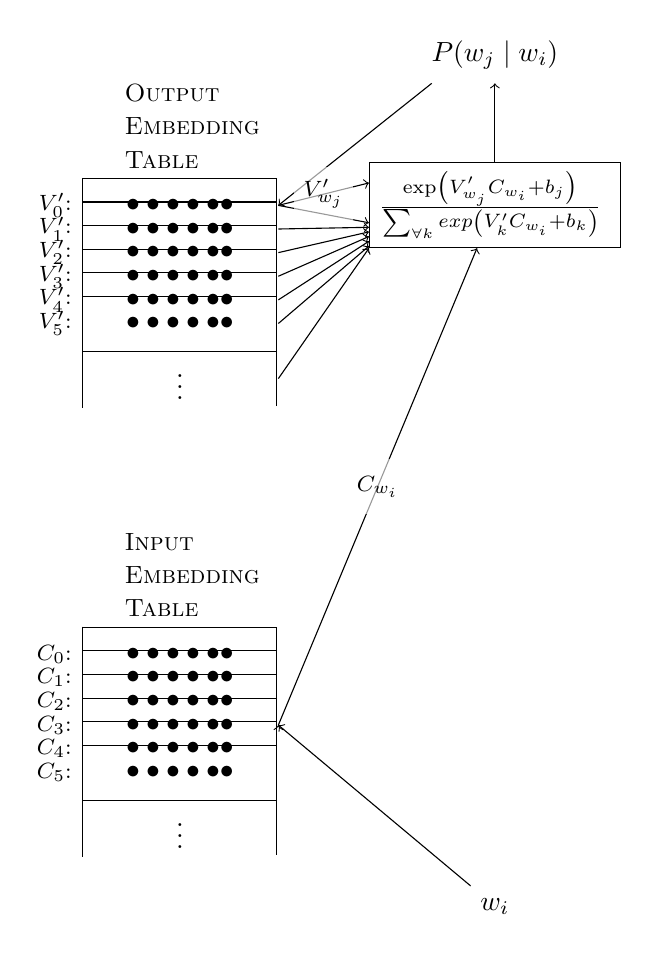
\begin{tikzpicture}[]


\node(w1) at (0,0) {$w_{i}$};


\node(Cn)[lookupbox] at (-4,1) {$\vdots$};
\def\tblmax{6}
\foreach \ii in {1,...,\tblmax} {
	\pgfmathsetmacro\pos{(\ii - 1) * 3 };
	\pgfmathtruncatemacro\jj{(\tblmax -\ii)};
	
	\node(C\ii)[lookupbox, above = \pos mm of Cn]{$\bullet\bullet\bullet\bullet\bullet\bullet$};
	\node(Clbl\ii)[left = 0mm of C\ii]{\footnotesize $C_\jj$:};
};
\node(C)[above = 0mm of C\tblmax.north, text width=40] {\small \textsc{Input \\Embedding Table}};


\draw[->] (w1) edge (C3.east);


\node(L2)[layer, above = 8 of w1]{
$\frac{\exp\left(V^\prime_{w_j} C_{w_i} + b_j \right)}%
{\sum_{\forall k}exp\left(V^\prime_{k} C_{w_i} + b_k \right)}$
};
\draw[->]  (C3.east) edge node[labe]{$C_{w_i}$} (L2);


\node(out)[above = of L2]{$P(w_j \mid w_i)$};
\draw[->] (L2) edge (out);

\node(Vn)[lookupbox, above = 5 of Cn] {$\vdots$};
\def\tblmax{6}
\foreach \ii in {1,...,\tblmax} {
	\pgfmathsetmacro\pos{(\ii - 1) * 3 };
	\pgfmathtruncatemacro\jj{(\tblmax -\ii)};
	
	\node(V\ii)[lookupbox, above = \pos mm of Vn]{$\bullet\bullet\bullet\bullet\bullet\bullet$};
	\node(Vlbl\ii)[left = 0mm of V\ii]{\footnotesize $V_\jj^\prime$:};
	
	\pgfmathsetmacro\ang{(\ii * -2 + -180+20 };
	\draw[->] (V\ii.east) -- (L2.\ang);
};

\draw[->] (Vn.east) -- (L2.south west);
\node(C)[above = 0mm of V\tblmax.north, text width=40] {\small \textsc{Output \\Embedding Table}};


\draw[->] (out.204) -- (V6.east);
\draw[->] (V6.east)-- node[labe]{$V_{w_j}^\prime$} (L2.170);

\end{tikzpicture}

\end{document}